\documentclass[conference]{IEEEtran}
\IEEEoverridecommandlockouts
% The preceding line is only needed to identify funding in the first footnote. If that is unneeded, please comment it out.
\usepackage{cite}
\usepackage{amsmath,amssymb,amsfonts}
\usepackage{algorithmic}
\usepackage{graphicx}
\usepackage{textcomp}
\usepackage{xcolor}
\def\BibTeX{{\rm B\kern-.05em{\sc i\kern-.025em b}\kern-.08em
    T\kern-.1667em\lower.7ex\hbox{E}\kern-.125emX}}
\begin{document}

\title{Course Project Final Report\\

}

\author{\IEEEauthorblockN{Clayton Tucker}
\IEEEauthorblockA{\textit{COSC325} \\
\textit{Ctrl Alt Delete}\\
Knoxville, US \\
ctucke24@vols.utk.edu}
\and
\IEEEauthorblockN{Todd Van Meter}
\IEEEauthorblockA{\textit{COSC 325} \\
\textit{Ctrl Alt Delete}\\
Knoxville, US \\
tvanmete@vols.utk.edu}
\and
\IEEEauthorblockN{Danyil Chuprynov}
\IEEEauthorblockA{\textit{COSC 325} \\
\textit{Ctrl Alt Delete}\\
Knoxvile, US \\
dchupryn@vols.utk.edu}
\and
\IEEEauthorblockN{Ian Henson}
\IEEEauthorblockA{\textit{COSC 325} \\
\textit{Ctrl Alt Delete}\\
Knoxvile, US \\
tkd995@vols.utk.edu}
}

\maketitle

\begin{abstract}
This document is a model and instructions for \LaTeX.
This and the IEEEtran.cls file define the components of your paper [title, text, heads, etc.]. *CRITICAL: Do Not Use Symbols, Special Characters, Footnotes, 
or Math in Paper Title or Abstract.
\end{abstract}

\begin{IEEEkeywords}
component, formatting, style, styling, insert
\end{IEEEkeywords}

\section{Introduction}
Predicting stock prices is a challenging yet critical task in finance due to market volatility and unpredictability. Machine learning provides powerful tools capable of identifying complex patterns within historical financial data, which can lead to more accurate stock price forecasts.

We aim to specifically examine the application of machine learning techniques to predict the stock prices of Berkshire Hathaway, a leading investment firm known for its diverse portfolio and market influence [1]. Accurate prediction models for Berkshire Hathaway's stock could significantly assist investors in making informed decisions, managing investment risks, and capitalizing on market trends.

Utilizing the Berksire-Hathaway historical stock data from Kaggle, we aim to:
\begin{itemize}
    \item Analyze and pre-process historical data to identify predictive features.
    \item Implement and evaluate multiple ML models to determine their forecasting accuracy.
    \item Assess the practical effectiveness of ML in predicting Berkshire Hathaway’s stock performance.
\end{itemize}

Through these objectives, the project seeks to contribute to improving investment strategies and demonstrating the value of ML applications in financial market analysis.

\section{Data Exploration}

\subsection{The Dataset}

The dataset used in this study is the Berkshire Hathaway Stock Price Data, sourced from Kaggle (Haddi, 2023). This dataset includes historical stock information consisting of 1,671 daily samples collected from January 2, 2020, to July 29, 2024. Each sample contains eight features: open price, high price, low price, close price, adjusted close price, trading volume, log-transformed closing price, and date converted to an ordinal number format. The dataset is continuous and inherently balanced as it involves time-series data rather than categorical classes. Due to its nature, it requires special pre-processing techniques, such as stationary adjustments and log transformations, to ensure effective application of predictive models.

\subsection{Preprocessing}
Detailed preprocessing steps applied to the data included:
\begin{itemize}
    \item Filtering to include only data from January 2020 onwards to maintain consistency and relevance.
    \item Handling missing values by forward-filling daily gaps to maintain continuity, ensuring no temporal discontinuities in the dataset.
    \item Transforming the 'Close' price feature using a logarithmic scale to stabilize variance and manage heterogeneity of variance.
    \item Calculating the first-order differences on all features to achieve stationarity, a requirement for ARIMA modeling, confirmed through the Augmented Dickey-Fuller (ADF) test.
    \item Then a moving average and standard deviation features was calculated to improve accuracy, the latter was required for ARIMA.
\end{itemize}

The preprocessing steps above were critical to improving and ensuring the effectiveness of the predictive models employed in this study.

\subsection{Data Analysis}\label{AA}
\begin{itemize}
    \item \textbf{Overall Stock Price Trend}: Berkshire Hathaway's stock price exhibited an increasing trend over the analyzed period from January 2020 to July 2024. The closing price started around \$228 in early 2020 and rose significantly, reaching approximately \$438 in July of 2024, suggesting overall growth and positive long-term performance.
    \item \textbf{Seasonality and Stationarity}: Initial tests for stationarity ADF test indicated non-stationarity in raw closing prices (Test Statistic: -0.52, P-Value: 0.89). Thus, data transformations (log differences) were applied to make the dataset stationary, which is essential for effective ARIMA modeling.
    \item \textbf{Volume Insights}: The daily traded volume shows significant variability, indicating periods of increased investor activity. The high volatility in trading volume suggests events or news that significantly influenced investor behavior and stock prices.
    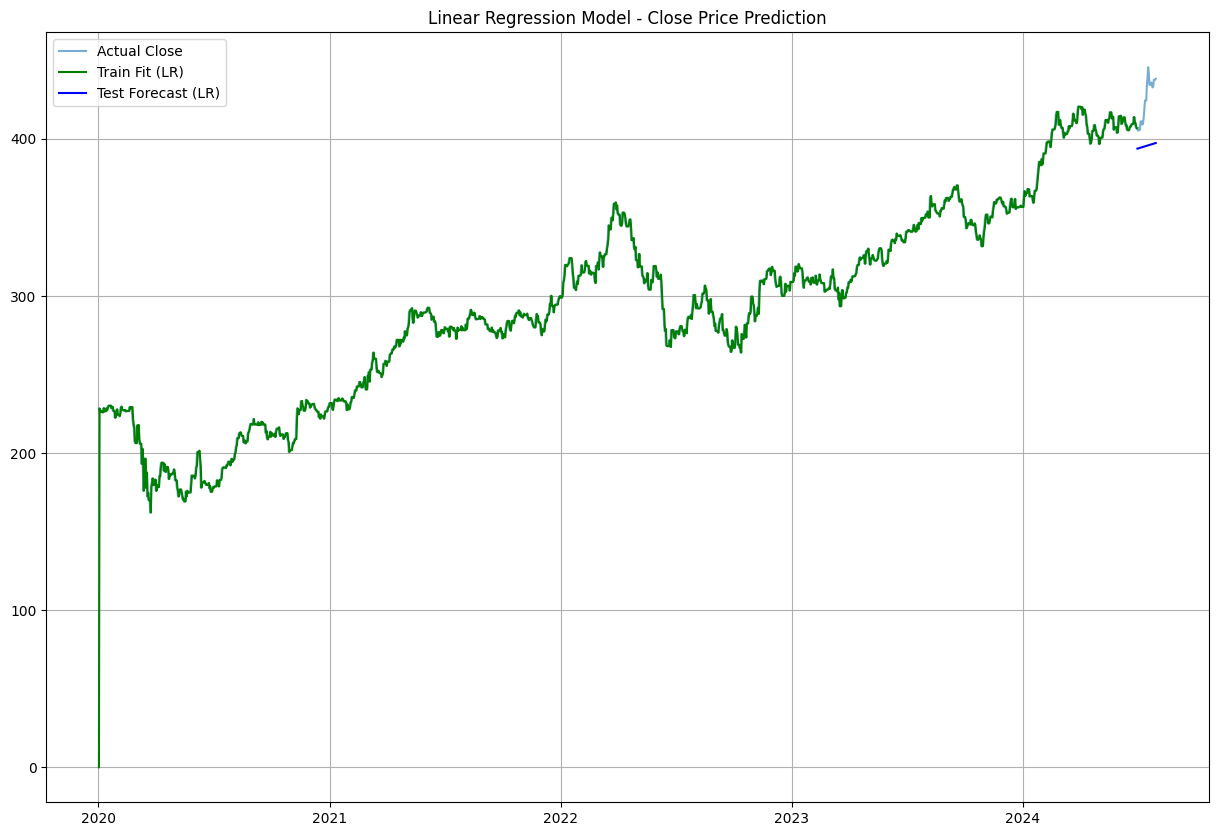
\includegraphics[scale=0.25]{screenshots/linreg.png} %screenshots/linreg.png
    \item \textbf{Model Performance Comparison}: ARIMA and Random Forest models produced similar predictive accuracy (RMSE approximately 22.2 and 22.1, respectively), outperforming Linear Regression, which had notably higher errors (RMSE approximately 31.6). This confirms non-linearity in stock price data and highlights the effectiveness of non-linear models like ARIMA and Random Forest.
    \\
     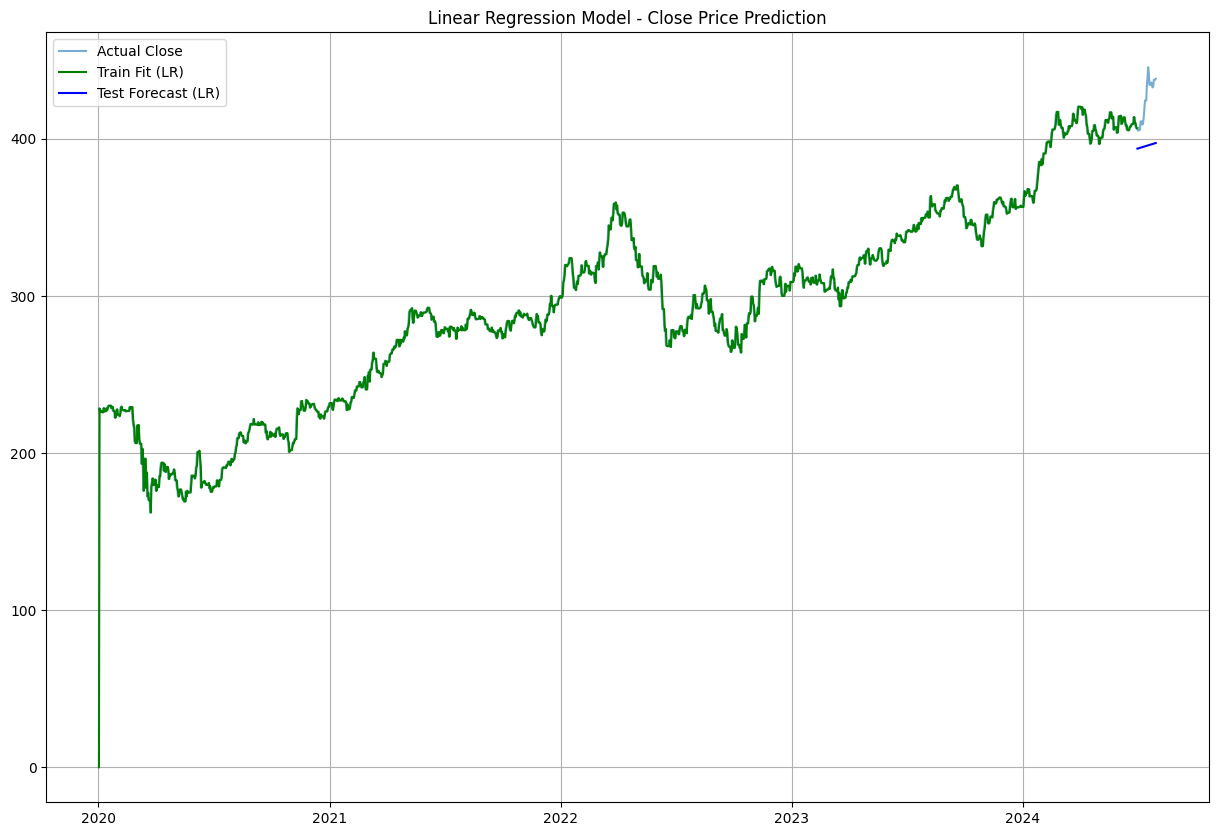
\includegraphics[scale=0.125]{screenshots/linreg.png} %screenshots/linreg.png
      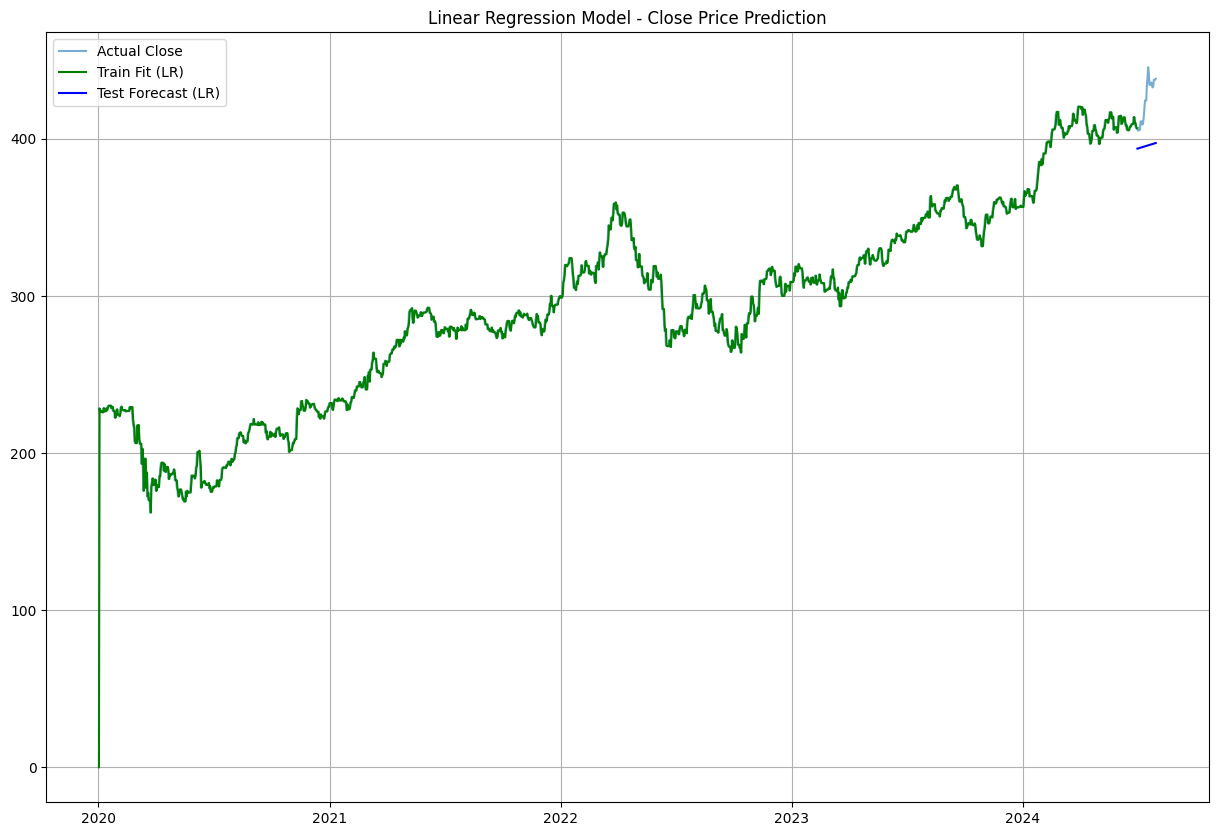
\includegraphics[scale=0.125]{screenshots/linreg.png} %screenshots/ranfor.png
       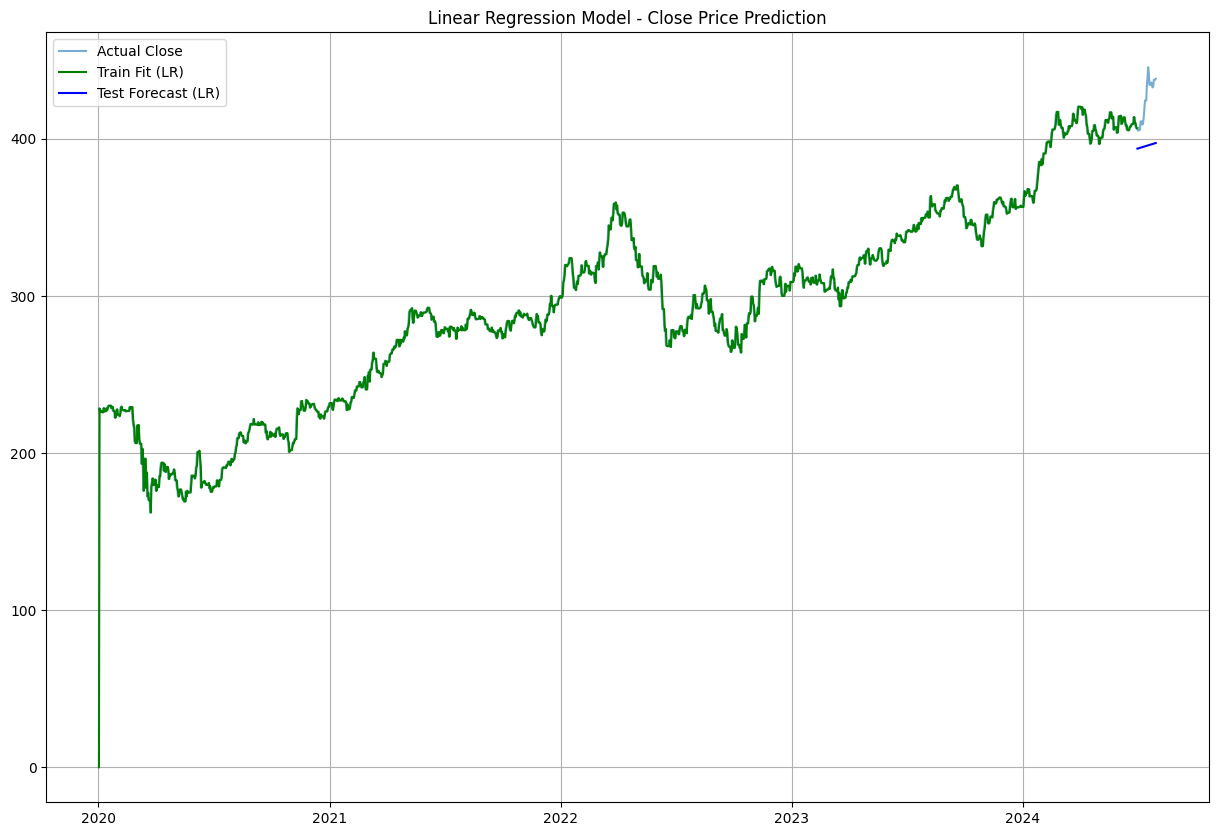
\includegraphics[scale=0.125]{screenshots/linreg.png} %screenshots/arima.png
    \item \textbf{Error Analysis}: Both ARIMA and Random Forest displayed relatively low and similar absolute errors (~18), indicating that while there are predictive limitations, both models adequately captured short-term movements in stock prices.
    \item \textbf{Possible Overfitting with Random Forest}: Random Forest exhibited consistent predictions across test days (constant values), suggesting possible overfitting to the training data. While it resulted in low errors, the model’s predictions lacked variability, potentially limiting its usefulness in dynamic real-world trading scenarios.
\end{itemize}

\section{Baseline Model}

Before we can process our dataset, we must first decide the best possible model as our baseline. As there are many different baselines, all with their strengths and weaknesses, we explored some of the existing solutions to determine which one to use.

\subsection{Existing Solutions}

\begin{itemize}

    \item \textbf{Linear Regression}: Linear Regression is a simple model that people have used for stock market predictions. However, after using a Linear Regression model on our data, our predictions were linear and flat. This is likely due to our data being nonlinear, making Linear Regressions an unideal model to use.   

    \item \textbf{Random Forests}: Another popular model used in stock market predictions is Random Forests. Random Forests, compared to Linear Regression, is capable of handling non-linear data and provides better results such as a lower MSE. There is some drawbacks, as random forests struggles with time series data.

    \item \textbf{ARIMA}: ARIMA models are also well known in stock market predictions and considered one of the best among other models[1]. Just like Random Forests, ARIMA models can handle non-linear data, but requires the data to be stationary for best performance. 

    \item \textbf{Moving Average}: Moving Average is another consideration as they have been widely used before. They are known being able to be tailored to different time-frames and smoothing price-data, but requires extra implementations, such as a Regression model, to fine-tune signal delays[2].

\end{itemize}

\subsection{Baseline Model}

We used a Manual ARIMA Model as our baseline for this project. Compared to other known solutions, ARIMA is known for providing better results and being more accurate.

\begin{itemize}

    \item \textbf{Performance}:  \\
    \includegraphics[scale=0.30]{ARIMA.png} %put a picture of the ARIMA model

    \item \textbf{Further Analysis}:
    The baseline model offered several benefits, such as being able to handle data non-stationary, auto regress on past values, and eliminate the need for external values. However, the model also came with its own issues. The predictions line became linear, indicating that our model is most likely oversimplified, and the model struggled with sudden shocks, such as the COVID-19 pandemic.

\end{itemize}

\section{Model Improvements}

\section{Distribution of Work}

\begin{thebibliography}{00}
\bibitem{b1} Umer Haddii, “Berkshire Hathaway Stock Price Data,” Kaggle.com, 2024. https://www.kaggle.com/datasets/umerhaddii/berkshire-hathaway-stock-price-data

\end{thebibliography}

\end{document}


